%\documentclass[notes=onlyslideswithnotes]{beamer}
%\documentclass[handout]{beamer}

\documentclass{beamer}
\usetheme{Berlin}
%\usecolortheme[rgb={0.65,0.15,0.25}]{structure}
\usefonttheme[onlymath]{serif}
\usepackage[latin1]{inputenc}
\usepackage{color}
\usepackage{amsmath}
\usepackage{amssymb}
\usepackage{amsfonts}
\usepackage[all]{xy}
\usepackage{graphicx}
\beamertemplatenavigationsymbolsempty
\def\1{1\!{\rm l}}
\newcommand{\argmin}[1]{\underset{#1}{\mathrm{Argmin} \ }}
\newcommand{\Bcal}{\mathcal{B}}
\newcommand{\Ccal}{\mathcal{C}}
\newcommand{\Dcal}{\mathcal{D}}
\newcommand{\Ecal}{\mathcal{E}}
\newcommand{\Gcal}{\mathcal{G}}
\newcommand{\Mcal}{\mathcal{M}}
\newcommand{\Ncal}{\mathcal{N}}
\newcommand{\Pcal}{\mathcal{P}}
\newcommand{\Qcal}{\mathcal{Q}}
\newcommand{\Lcal}{\mathcal{L}}
\newcommand{\Tcal}{\mathcal{T}}
\newcommand{\Ucal}{\mathcal{U}}
\newcommand{\alphabf}{\mbox{\mathversion{bold}{$\alpha$}}}
\newcommand{\betabf}{\mbox{\mathversion{bold}{$\beta$}}}
\newcommand{\gammabf}{\mbox{\mathversion{bold}{$\gamma$}}}
\newcommand{\mubf}{\mbox{\mathversion{bold}{$\mu$}}}
\newcommand{\thetabf}{\mbox{\mathversion{bold}{$\theta$}}}
\newcommand{\Pibf}{\mbox{\mathversion{bold}{$\Pi$}}}
\newcommand{\psibf}{\mbox{\mathversion{bold}{$\psi$}}}
\newcommand{\Sigmabf}{\mbox{\mathversion{bold}{$\Sigma$}}}
\newcommand{\taubf}{\mbox{\mathversion{bold}{$\tau$}}}
\newcommand{\Ebf}{{\bf E}}
\newcommand{\Cbf}{{\bf C}}
\newcommand{\Gbf}{{\bf G}}
\newcommand{\Hbf}{{\bf H}}
\newcommand{\Ibf}{{\bf I}}
\newcommand{\mbf}{{\bf m}}
\newcommand{\Obf}{{\bf 0}}
\newcommand{\Rbf}{{\bf R}}
\newcommand{\Sbf}{{\bf S}}
\newcommand{\Tbf}{{\bf T}}
\newcommand{\Ubf}{{\bf U}}
\newcommand{\Vbf}{{\bf V}}
\newcommand{\xbf}{{\bf x}}
\newcommand{\Xbf}{{\bf X}}
\newcommand{\Wbf}{{\bf W}}
\newcommand{\Ybf}{{\bf Y}}
\newcommand{\Zbf}{{\bf Z}}
\newcommand{\Esp}{{\mathbb E}}
\newcommand{\Var}{{\mathbb V}}
\newcommand{\Cov}{{\mathbb C}\mbox{ov}}
\newcommand{\Ibb}{{\mathbb I}}
\newcommand{\Rbb}{\mathbb{R}}
\newcommand{\biz}{\begin{itemize}}
\newcommand{\eiz}{\end{itemize}}
\newcommand{\bcent}{\begin{center}}
\newcommand{\ecent}{\end{center}}
\newcommand{\barr}{\begin{array}}
\newcommand{\earr}{\end{array}}
\newcommand{\btab}{\begin{tabular}}
\newcommand{\etab}{\end{tabular}}
\newcommand{\ben}{\begin{enumerate}}
\newcommand{\een}{\end{enumerate}}
\newcommand{\bdes}{\begin{description}}
\newcommand{\edes}{\end{description}}
\newcommand{\dps}{\displaystyle}
\newcommand{\la}{\lambda}
\newcommand{\bqas}{\begin{eqnarray*}}
\newcommand{\eqas}{\end{eqnarray*}}
\newcommand{\noi}{\noindent}
\newtheorem{Prop}{Proposition}
\newtheorem{Propri}{Propri\'et\'es}

\definecolor{darkblue}{rgb}{0,0,0.55}
\definecolor{darkgreen}{rgb}{0,0.55,0}
\definecolor{darkred}{rgb}{0.75,0,0}
\definecolor{rougeF}{rgb}{0.65,0.15,0.25}
\newcommand{\noir}[1]{\textrm{\textcolor{black}{#1}}}
\newcommand{\argmax}[1]{\underset{#1}{\mathrm{Argmax} \ }}

\newcommand{\coul}[1]{\textcolor{rougeF}{#1}}

\title[Segmentation and Model Selection]{Segmentation and
Model Selection}
\author[]{C. Berard, A. C�lisse, J.-J.Daudin, E. Lebarbier, \\
M.-L. Martin-Magniette, T. Mary-Huard, G. Rigaill, \\
S. Robin, B. Thiam, A. Urbain}





\date{February 10, 2009}

\begin{document}

\frame{\titlepage}
%

%======================
\frame{ \frametitle{ Segmentation for CGH microarrays
data analysis}


{\small

\begin{tabular}{cc}

  \begin{tabular}{p{3.5cm}} \textcolor{blue}{CGH Objective:} Detection of chromosomal aberrations (within chromosome) \end{tabular} &
  \begin{tabular}{c}
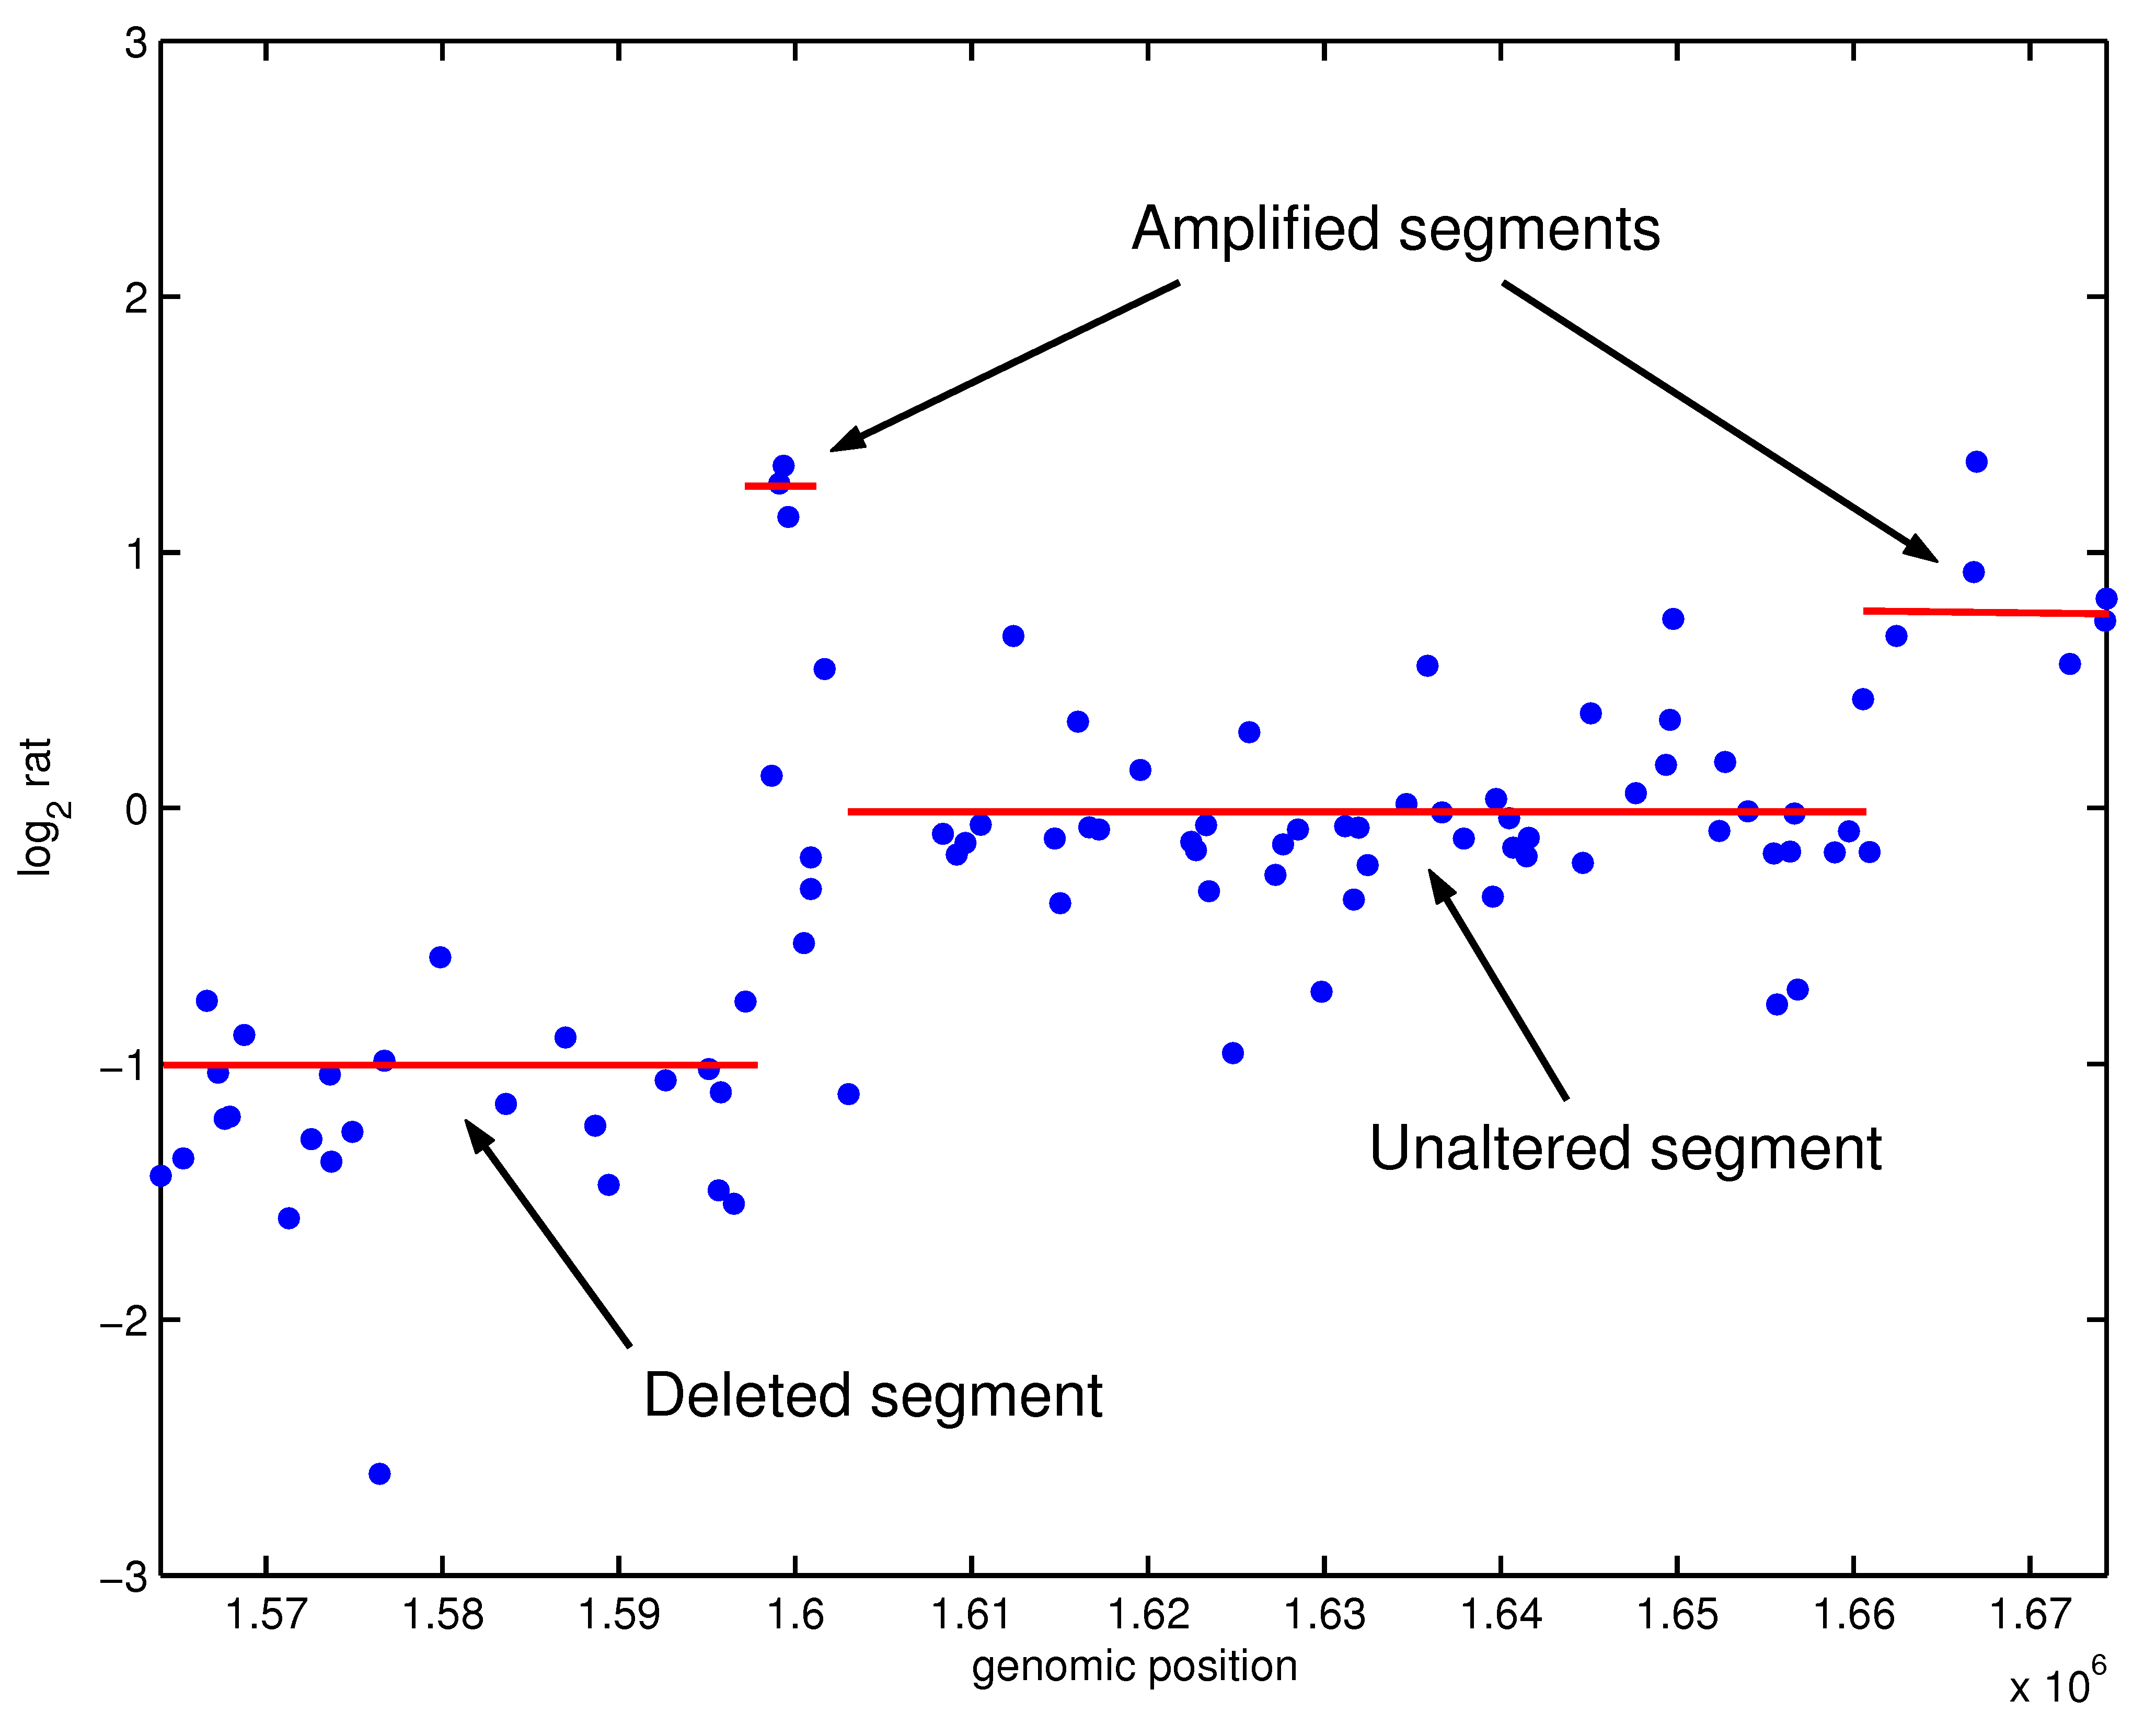
\includegraphics[scale=0.3]{profile_example.png}
  \end{tabular}
\\

 & \begin{tabular}{p{5cm}} A dot on the graph represents \\

  $
   \footnotesize{
   \log_2 \left\{ \frac{\text{ $\sharp$ copies of BAC(t) in the test
          genome }}{\text{$\sharp$ copies of BAC(t) in the reference
          genome}}\right\}}
  $ \end{tabular} \\

  \end{tabular}

  }
}
%======================
\frame{ \frametitle{ Segmentation Model for on signal}


{\small
\noindent \textcolor{blue}{Model.} The observed signal
$Y=(Y_1,\ldots,Y_n)$ is such that:
$$
Y_t=\mu_k + E_t \ \ \ \  \mbox{ if position $t$ is in segment
$I_k=[t_{k-1}+1,t_{k}]$,}
$$
with $\{E_t\}$ i.i.d. $\sim \Ncal(0,\sigma^2)$ and $k=1,\ldots,K$.

\vspace{.4cm}

\noindent \textcolor{blue}{The parameters} are { \footnotesize $T_K =
(t_1, ..., t_{K-1})$, $\theta_K  = (\mu_1,\hdots,\mu_K,\sigma^2)$ and $K$.}

\vspace{.4cm}

\noindent \textcolor{blue}{Parameter estimation by maximum
likelihood.} For a fixed K,

$$
(\hat{T}_K,\hat{\theta}_K)= \argmax{(T_K,\theta_K)} \mathcal{L}_K(Y;T_K, \theta_K)
$$



$\rightarrow$ a dynamic programming is used to find the breakpoints.


%\vspace{-0.5cm}
 \footnotesize {\hspace{5cm} \emph{Picard \& al., BMC
Bioinformatics, 2005}}

}
}

%======================
\frame{ \frametitle{Model Selection: different approaches}
\vspace{-0.2cm}

{ \footnotesize


$\bullet$ \textcolor{blue}{Penalized criterion} in the case
$\sigma^2$ known.

\vspace{-0.3cm}
\begin{equation*}
\hat{K} = \argmin{K} \underbrace{\sum_{k=1}^K \sum_{t \in \hat{I}_k}
(y_t-\hat{\mu}_k)^2}_{\text{$\hat{R}_K$: Fit}} +
\underbrace{\sigma^2 \left (c_2 K + c_1\log(\mathrm{C}_n^K) \right
)}_{\text{Penalty}} \ \ \mbox{with $c_1=2$ and $c_2=5$}
\end{equation*}

To ensure: \vspace{-0.4cm}


$$
E\|s-\hat{s}\|_n^2 \leq C\log(n)\times\inf_{T}E\|s-\hat{s}_{T}\|_n^2
\ \  \ \ \mbox{if $s=\sum_{k=1}^K \mu_k\mathbb{I}_{I_k}$}
$$

\hspace{6cm} \emph{Lebarbier, Signal Processing,
2005} \\

%\vspace{0.3cm}


$\bullet$ \textcolor{blue}{Resampling} in the case
$\sigma^2=\sigma^2 / \sigma^2_t$.

\vspace{-0.3cm}
%\begin{tabular}{p5cm}
\begin{equation*}
\hat{K} = \argmin{K} \underbrace{ \frac{1}{V}\sum_{v=1}^V
\hat{R}_K^{v}}_{\text{V. fold version of $\hat{R}_K$}}
\end{equation*}

Robust to $\rightarrow$ heteroscedasticity

\hspace{1.34cm} $\rightarrow$ distribution of $\{E_t\}$

}




}


%======================
\frame{ \frametitle{ Model Selection}


{\small



%\vspace{-0.5cm} \hspace{11cm} \emph{C�lisse \& Arlot, 2008} \\
$\bullet$ \textcolor{blue}{A new BIC criterion} in the case
$\sigma^2=\sigma^2 / \sigma^2_k$.

\vspace{-0.6cm}

\begin{equation*}
\hat{K} = \argmin{K} - 2 \log{\left ( \sum_{T_K}
\mathcal{L}_K(Y;T_K, \hat{\theta}_K) \right )} + K \log{(n)}-2 \log{
(P(T|K) P(K))}
\end{equation*}

with for example $P(T|K)=1/\mathrm{C}_n^K$

\vspace{0.2cm}

$\rightarrow$ We can obtain the breakpoints/segments probabilities

\vspace{.5cm}

\noindent \textcolor{blue}{The {\sc select} group:} a collaboration between 4 groups:\\
$\bullet$ Laboratoire Probabilit�s et Statistiques de Paris XI \\
$\bullet$ SELECT INRIA FUTUR Team \\
$\bullet$ Statistique et G�nome Team \\
$\bullet$ Universit� Paris Descartes


}
}
%======================
\frame{ \frametitle{ A new Segmentation/Clustering Model}

{\small
\textcolor{blue}{Objective.} Provide a biological status of the
detected segments: normal/deleted/amplified.


%\begin{figure}
%  \includegraphics[scale=.4]{nouveau_model.png}
%\end{figure}



%$$
%\begin{tabular}{cc}
%  \includegraphics[scale=.3]{FigSegClas-1.png} &
%  \includegraphics[scale=.3]{FigSegClas-2.png} \\
%Segmentation &  Segmentation/Clustering
%\end{tabular}
%$$

}
}

%======================
\frame{ \frametitle{ A new Segmentation/Clustering Model}


{\small
\textcolor{blue}{Model:} a mixture model for the segments $Y^k$ with size $n_k$

\[Y^k|Z_p^k=1 \sim \mathcal{N}(m_p \1_{n_k},s_p^2 I_{n_k}) \ \ \  p=1,\ldots,P \]


\vspace{0.5cm}

\textcolor{blue}{Parameter estimation.} A DP-EM algorithm
\begin{enumerate}
\item When $T$ is known, the EM algorithm is used to estimate $\theta$

\item When $\theta$ is known, Dynamic programming is used to estimate $T$.

\end{enumerate}


\vspace{0.5cm}

\textcolor{blue}{Model Selection:} choice of $2$ parameters $P$ and $K$.

{ \footnotesize \hspace{6cm} \emph{Picard \& al., Biometrics, 2007}}
}

}


%======================
\frame{ \frametitle{ A Mixed linear model with breakpoints}

\vspace{-0.4cm}

{\small

\hspace{-1cm}
\begin{tabular}{cc}
  \begin{tabular}{p{6cm}}


\vspace{0.2cm}

Consider the profiles of $M$ patients, we look for \\

\vspace{0.2cm}


$\rightarrow$ \textcolor{blue}{patient-specific segmentation} \\

$\rightarrow$ accounting a (random) \textcolor{blue}{probe effect
$U_t$} that induces correlations between profiles of patients
at same position. \\ \\

 \textcolor{blue}{Probe quality or other technical effect} may alter all the profiles at the same
    position. \\ \\

{\footnotesize $ Y_{m t} = \mu_{m k} + U_{t} + E_{m t} \qquad \mbox{if $t
\in I_{m k}$}$}\\ \\
\mbox{\footnotesize where $\{U_{t}\}$ are i.i.d. $\sim
\Ncal(0,
\sigma^2_u)$, $\{E_{m t}\}$ are i.i.d. $\sim \Ncal(0, \sigma^2)$,}\\
{\footnotesize $\{U_{t}\}$ and $\{E_{m t}\}$ are independent}

  \end{tabular}
  &
  \begin{tabular}{p{4cm}}
    %\begin{figure}
    \includegraphics[scale=0.4]{MixSeg1.png}
  %  \end{figure}
  \end{tabular}
\end{tabular}

}

}

%======================
\frame{ \frametitle{ A Mixed linear model with breakpoints}

{\small
\textcolor{blue}{General model}
$$
\Ybf = \underset{\mbox{Segmentation}}{\underbrace{\Tbf \mubf}} +
\underset{\mbox{Random effect}}{\underbrace{\Zbf \Ubf}} + \Ebf
$$


\vspace{.5cm}
\textcolor{blue}{Parameter estimation}


$\bullet$ The model can be viewed as model with
incomplete data:
\textcolor{blue}{$U$ is hidden} \\

$\bullet$ E-M strategy:

\hspace{2cm} $\rightarrow$ E step. The unobserved effect $U$ is predicted



\hspace{2cm} $\rightarrow$ M step. The segmentation is done using the DP
\begin{eqnarray*}
\widehat{\Tbf \mubf} & = & \arg\min_{\Tbf\mubf} \|\Ybf -
{\Tbf\mubf}-\Zbf \widehat{\Ubf})\|^2.
\end{eqnarray*}

%\textcolor{blue}{Practical
%implementation: the segmentation step.} The  step is computationally
%heavy.


%\hspace{2cm} $\rightarrow$ A new two-stage dynamic programming
%algorithm: an \textcolor{blue}{optimal} procedure with a reduced
%complexity $\mathcal{O}( \lambda L n^2 (n+\lambda L^2))$ ($\lambda
%<< 1$).

}
}


%======================
\frame{ \frametitle{ A new two-stage Dynamic Programming procedure}

{\small
\textcolor{blue}{We have to}
\begin{equation*}
\min_{\{\Tbf,\mubf\}} RRS_{K}(\mubf, \Tbf)= \min_{K_1+\ldots+K_L=K}
\left \{  \sum_{l=1}^L \min_{\Tbf_l,\mubf_l} RSS^l_{K_l}
(\Tbf_l,\mubf_l) \right \}
\end{equation*}


\textcolor{blue}{Proposed strategy.}
\begin{description}
\item[Stage-1] each profile $l$ is segmented into $K_l$
segments.
\begin{eqnarray*}
\forall l \in [1:L] \ \ \{\hat{\Tbf}_l,\hat{\mubf}_l\}=
\min_{\Tbf_l,\mubf_l} RRS_{K_l}^l.
\end{eqnarray*}


\item[Stage-2] the second step consists in solving:
\begin{eqnarray*}
\min_{K_1+\ldots+K_L=K} \left \{  \sum_{l=1}^L RRS^l_{K_l}
(\hat{\Tbf}_l,\hat{\mubf}_l) \right \}
\end{eqnarray*}
The principle of this stage is to spread $K$ segments among $L$
patients.
\end{description}

}
}


%======================
\frame{ \frametitle{ Diffusion and many application
fields}


{\small

\noindent \textcolor{blue}{Contribution to the diffusion:}\\
$\bullet$  Workshop "Change-Point Detection Methods and Application"
(Paris, Sept. 2008, organized with F. Picard, CNRS, Lyon)\\
$\bullet$ Packages R: Segclust available and CGHseg in construction

\vspace{.5cm}

\noindent \textcolor{blue}{Collaborations:}\\
$\bullet$ CGH (Institut Curie),\\
$\bullet$ Growth phase detection of trees (CIRAD Montpellier), \\
$\bullet$ Change detection in climate (CEFE-CNRS, LSCE-CEA)\\
$\bullet$  Change Detection in food for goats (AgroParisTech Paris)

}
}

%======================
\frame{ \frametitle{ Work in progress and perspectives}

{\small


$\bullet$ Generalization of the Segmentation/Clustering framework to the multivariate case

\vspace{.5cm}


$\bullet$ Model selection for the joint segmentation

$\rightarrow$ adapte the different model selection criteria in the multiple case by taking into account the correlation structure. \\

\vspace{.5cm}


$\bullet$ New size of data. With the use of tiling arrays, the size \\
of one signal is huge: $n \sim 10^6$\\

$\rightarrow$ Adapt the segmentation algorithm to the size of the data

$\rightarrow$ Account others dependencies


}

}

\end{document}
